\documentclass[12pt]{article}
\usepackage[utf8]{inputenc}
\usepackage[pdftex]{graphicx}
\usepackage{graphicx}       % front image
\usepackage{hyperref}       % links and email
\usepackage{indentfirst}
\usepackage{setspace}
\usepackage{anysize}
\usepackage{makeidx}
\usepackage[brazil]{babel}
\usepackage{eurosym}
\usepackage{pbox}           % linebreaks in tables
\usepackage{geometry}           
\usepackage{tabularx}           
\usepackage[table]{xcolor}
\usepackage{booktabs}

\geometry{verbose,tmargin=1.5cm,bmargin=1.5cm,lmargin=1.5cm,rmargin=1.5cm}

% footnotes in tables
\usepackage{footnote}
\makesavenoteenv{tabular}

% auto update years
\usepackage{datenumber}
\newcounter{dateone}
\newcounter{datetwo}
\newcommand{\difftoday}[3]{%
      \setmydatenumber{dateone}{\the\year}{\the\month}{\the\day}%
      \setmydatenumber{datetwo}{#1}{#2}{#3}%
      \addtocounter{datetwo}{-\thedateone}%
      \the\numexpr-\thedatetwo/365\relax
}

% opening
\title{Plano de Negócio\\Seven Keys}
\author{Paulo Markes\\Game Designer - Gerente}

\begin{document}
\begin{titlepage}
    \centering
    \maketitle
    \thispagestyle{empty}   % discard page number
    
\includegraphics[width=10cm]{7keys.png}
    \vfill
    {\raggedright
    ManaTeam Entertainment\\
    \href{mailto:manateamentertainment@gmail.com}{manateamentertainment@gmail.com}\\
    }
\end{titlepage}

\begin{abstract}
Este documento visa apresentar o plano de negócio para o desenvolvimento do jogo Seven Keys, apresentando o foco do desenvolvimento desse jogo, os custos envolvidos em sua produção
público-alvo entre outros aspectos importantes para o desenvolvimento.
\end{abstract}

\pagebreak
\tableofcontents
\pagebreak

\section{Triângulo de Prioridades}

O triângulo de prioridades representa as três prioridades principais do projeto. O projeto será focado no tempo, pois o custo total para realização do jogo será fixo e irrisório e o escopo irá oscilar em relação ao tempo.

\begin{figure}[ht]
\centering
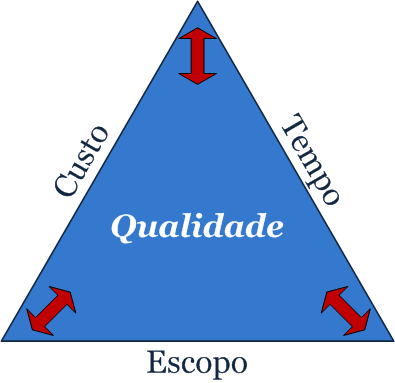
\includegraphics[width=5cm]{3_restricoes.png}
\caption{Triângulo de Prioridades}
\label{fig:restricoes}
\end{figure}

Ainda sobre o tempo, o projeto terá uma duração de 4 meses, ou seja, o desenvolvimento deverá
ser rápido o suficiente para que a equipe consiga finalizar o jogo dentro do prazo estipulado, sem
deixar a qualidade de lado, buscando aprimoração sempre. \\

No entanto, mesmo com curto prazo de tempo, o jogo conterá diversas funcionalidades, descritas no GDD e no documento de Visão.
\section{Plataformas}

As plataformas suportadas, inicialmente, serão Windows e Linux.
O Linux possui um grande suporte de bibliotecas e ferramentas de desenvolvimento de software e o Windows possui uma grande base de usuários jogadores, fazendo com que ambas os sistemas operacionais se tornem alvos para o jogo.


\section{Público-alvo}
Pessoas acima de 16 anos, que sejam capazes de compreender a ideia do jogo e não se sintam
desconfortáveis por conta da história e dinâmica do jogo.

\section{Estratégia de divulgação}

O jogo TerraCota será divulgado nas seguintes mídias:
\begin{itemize}
  \item Redes sociais:
  \begin{itemize}
    \item Divulgação nas timelines dos desenvolvedores
    \item Divulgação nos grupos de desenvolvimento de jogos independentes, exemplo Indie Developers Brasil, Boteco Gamer, GameDev-DF, BRING, etc.
  \end{itemize}
  \item Fóruns de jogos eletrônicos
  \item Steam Greenlight
\end{itemize}

\section{Recursos disponíveis}

Os recursos disponíveis para o desenvolvimento contam com uma equipe de sete pessoas, sendo três desenvolvedores, três artistas e um músico, também contam os equipamentos usados por cada membro da equipe. A seguir é apresentada uma tabela com os dados financeiros relacionados aos recursos disponíveis.

\begin{table}[h]
\centering
\begin{tabular}{|l|l|l|l|l}
\cline{1-4}
\multicolumn{1}{|c|}{\textbf{Recursos}} & \multicolumn{1}{c|}{\textbf{Quantidade}} & \multicolumn{1}{c|}{\textbf{Valor Unitário}} & \multicolumn{1}{c|}{\textbf{Valor Total}} &  \\ \cline{1-4}
Notebooks                               & 7                                        & R\$ 2.500,00                                  & R\$ 17.500,00                             &  \\ \cline{1-4}
Sublime Text 3                          & 3                                        & R\$ 212,10                                   & R\$ 636,30                                &  \\ \cline{1-4}
Linux                                   & 3                                        & R\$ 0,00                                     & R\$ 0,00                                  &  \\ \cline{1-4}
Windows 8                               & 4                                        & R\$ 359,00                                   & R\$ 1.436,00                              &  \\ \cline{1-4}
*Adobe Ilustrator CC                    & 3                                        & R\$ 176,00                                   & R\$ 528,00                                &  \\ \cline{1-4}
*Adobe Photoshop CC Fotografia          & 3                                        & R\$ 88,00                                    & R\$ 264,00                                &  \\ \cline{1-4}
*Adobe After Effects CC &1 &R\$ 44,00 & R\$ 44,00
& \\ \cline{1-4}
Publicação na Steam Greenligth          & 1                                        & R\$ 304,12                                   & R\$ 304,12                                &  \\ \cline{1-4}
Mesa Digital &4  & R\$300,00  & R\$ 1200,00
& \\ \cline{1-4}
\multicolumn{3}{|c|}{\textbf{Total}}                                                                                              & R\$ 21.912,42                             &  \\ \cline{1-4}
\end{tabular}
\caption {Recursos de Hardware e Software}
\end{table}

\textit{* Os valores desses produtos são pagos por mês, a conta já converte o valor para 4 meses de uso.}
\\
\\
\\
\\
\\
\\

\begin{table}[h]
\centering
\begin{tabular}{lcrcr}
\toprule
\textbf{Recursos} & \textbf{Qtd} & \textbf{Valor/Hora} & \textbf{Horas} &
\textbf{Total} \\
\midrule
Desenvolvedor & 3 & R\$ 18,00 & 1920 & R\$ 103.680,00 \\
\rowcolor[gray]{0.9}
Designer Gráfico & 3 & R\$ 13,00 & 1920 & R\$ 74.880,00 \\
Músico & 1 & R\$ 13,00 & 600 & R\$ 7.800,00\\
\midrule
\rowcolor[gray]{0.7}
\multicolumn{4}{r}{\textbf{Total}} & R\$ 186.360,00\\
\bottomrule
\end{tabular}
\caption {Recursos Humanos}
\end{table}

\textit{* Os valores acima foram calculados considerando-se 40 horas de trabalho semanais em 4 meses de trabalho, com exceção do músico}
\\

Valor total do projeto: {\textbf{R\$ 208.272.42.}}

\section{Lucro esperado}

A equipe espera alcançar um lucros perto de 30\% em cima dos valores gastos para o desenvolvimento do jogo, para isso, é necessário se alcançar um valor em torno de R\$ 270.754,15 nas vendas, deixando assim todas as dívidas quitadas e mais R\$ 62.481.73 líquido.

\section{Número estimado de cópias a serem vendidas}

A seguir é apresentada uma tabela com determinados preços para o jogo e o número estimado de cópias que deveriam ser vendidas para se alcançar os lucros esperados, considerando também o custo do projeto. Os valores positivos são lucros além dos R\$ 270.754,15 (custo + lucro esperado). 

\begin{table}[h]
\centering
\begin{tabular}{|l|l|l|l|l}
\cline{1-4}
\multicolumn{1}{|c|}{\textbf{Valor do Jogo}} & \multicolumn{1}{c|}{\textbf{10k cópias vendidas}} & \multicolumn{1}{c|}{\textbf{15k cópias vendidas}} & \multicolumn{1}{c|}{\textbf{25k cópias vendidas}} &  \\ \cline{1-4}
R\$ 10,00                                    & R\$ -170.754.15                                        & R\$ -120.754,15                                        & R\$ -20.754.15                                     &  \\ \cline{1-4}
R\$ 15,00                                    & R\$ -170.754,15 &
R\$ -45.754,15                                        & R\$ 104.245,85                                     &  \\ \cline{1-4}
R\$ 20,00                                    & R\$ -70.754,15                                       & R\$ 29.245,85                                        & R\$ 229.245,85                                     &  \\ \cline{1-4}
\end{tabular}
\caption{Valores alcançados de acordo com o valor do jogo}
\end{table}

\section{Projeção do número de cópias a serem vendidas para recuperar o
	    investimento e para se obter o lucro esperado}

Pode-se notar na tabela com os valores apresentados as opções possíveis para as vendas do jogo. Para quitar os gastos do projeto e se obter o lucro esperado com uma meta de vendas para 15 mil cópias, o jogo deverá ter um valor de R\$ 18,00.
\end{document}
